\section{SAO}

\subsection{Algorithm}
To address the policy lag issue, SAO~\citep{hou2026single} proposes several modifications over the PPO-Clip objective to reach the following objective:

\begin{align}
     \label{eq:sao.obj}
     \max_{\theta}\;
     \Jcal_{\text{SAO}}(\theta)
     :=
     \Embb_{\tau \sim \pi_{\theta_{\text{rollout}}}}
     \left\{
         \sum_{t=0}^{T-1}
         \left[
             \operatorname{clip}\left(
                 \frac{\pi_{\theta}(a_t \mid s_t)}
                      {\pi_{\theta_{\text{rollout}}}(a_t \mid s_t)},
                 1-\epsilon_{\text{low}},
                 1+\epsilon_{\text{high}}
             \right)
             \hat{A}_{\phi}(s_t,a_t)
         \right]
         \log\pi_{\theta}(a_t \mid s_t)
     \right\},
\end{align}
where~\eqref{eq:sao.obj} is written in REINFORCE form~\eqref{eq:reinforce.obj}: the clipped importance ratio times the advantage is treated as a detached weight, and the explicit $\log\pi_{\theta}(a_t \mid s_t)$ term provides the policy-gradient direction.

\textbf{Remark}

\begin{enumerate}
    \item SAO drops the proximal policy $\pi_{\theta_{\text{old}}}$ and uses the behavior policy $\pi_{\theta_{\text{rollout}}}$ for importance sampling:
    \[
        r_t(\theta)
        =
        \frac{\pi_{\theta}(a_t\mid s_t)}
             {\pi_{\theta_{\text{rollout}}}(a_t\mid s_t)}.
    \]
    This also avoids recomputing probabilities under $\pi_{\theta_{\text{old}}}$ by reusing the log-probabilities generated during rollout.

    \item SAO applies a different trust region by clipping the rollout ratio to $[1-\epsilon_{\text{low}},1+\epsilon_{\text{high}}]$. As shown in \autoref{fig:sao.clip.region}, PPO clips by asking ``Has this sample already moved too far in the direction that appears beneficial?'', while SAO clips by asking ``Is the current policy still sufficiently close to the policy that generated this token for this sample to be trustworthy?''.
    \begin{itemize}
        \item \textbf{PPO's asymmetric construction is useful} when the advantage estimation is reliable, the data is fresh, the large ratio arose from parameter coupling or prior minibatch updates, and we want the sample to help undo an undesirable policy shift. For example, if $A=-1$ and $r=10$, PPO-Clip keeps the directionally corrective term $rA=-10$, which pushes the sampled action's probability down, while SAO clips it. Similarly, if $A=1$ and $r=0.1$, PPO keeps the corrective gradient, while SAO clips it. Because only one side is saturated for each advantage sign, PPO generally uses more of the batch and supports repeated minibatch optimization over collected data. However, PPO's retained corrective gradients can become dangerous in asynchronous or heavily off-policy training.
        \item \textbf{SAO's symmetric construction is helpful} in asynchronous or heavily off-policy training. For $A<0$ and $r\gg1$, the factor $rA$ can dominate a minibatch. That may be acceptable if $A$ is accurate and the sample is still relevant, but it can be destructive when the sample was generated by a substantially older actor, the trajectory context is highly off-policy, or one extreme token dominates the aggregate gradient. SAO bounds the importance ratio regardless of the advantage sign, giving direct control over this source of gradient heavy tails.
    \end{itemize}

    \begin{figure}[H]
        \centering
        \begin{minipage}{0.48\linewidth}
            \centering
            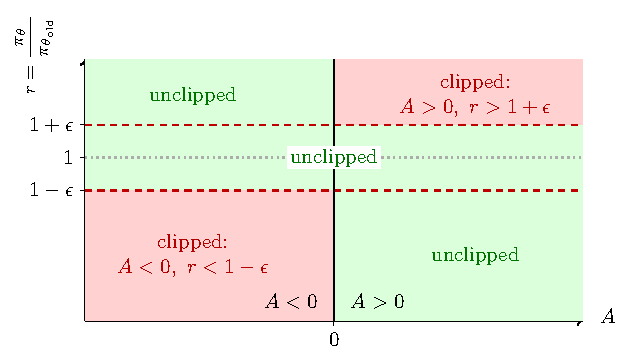
\includegraphics[width=\linewidth]{figures/ppo_clip_region.pdf}
            \centerline{\small PPO-Clip}
        \end{minipage}
        \hfill
        \begin{minipage}{0.48\linewidth}
            \centering
            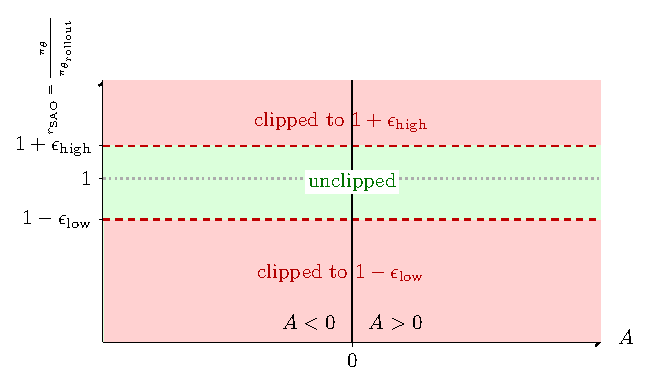
\includegraphics[width=\linewidth]{figures/sao_clip_region.pdf}
            \centerline{\small SAO-Clip}
        \end{minipage}
        \caption{PPO-Clip and SAO-Clip trust regions in the $(A,r)$ plane. PPO clips only in the regions selected by the clipped surrogate objective, while SAO directly clips the rollout-ratio $r=\frac{\pi_{\theta}(a_t|s_t)}{\pi_{\theta_{\text{rollout}}}(a_t|s_t)}$ to $[1-\epsilon_{\text{low}},1+\epsilon_{\text{high}}]$.}
        \label{fig:sao.clip.region}
    \end{figure}

    \item The strict two-sided gate has costs. First, once a token is outside the band, it gives no direct gradient, even when its advantage would have produced a restoring update. This is a distinction between filtering and constraining: SAO filters data; it does not project or roll the policy back into a feasible region. Second, importance sampling is unbiased only without truncation under the usual assumptions. PPO introduces bias through one-sided clipping, while SAO introduces more bias by dropping both tails. In particular, dropping a negative-advantage outlier can make the observed surrogate look artificially favorable because a large negative contribution has disappeared. Therefore, SAO's gated objective does not have PPO's uniform pointwise pessimism property. Third, clipping reduces the effective batch size: if many tokens leave the band, the nominal batch size may remain large while the number of contributing tokens collapses.

    \item The paper does not specify every detail of the advantage estimator $\hat{A}_{\phi}$. We sketch a consistent token-level interpretation below.
\end{enumerate}

\subsection{Guessed Advantage Estimator}

The main ambiguity is how to align token-level policy decisions, value estimates, rewards, and observations in a serialized agent trajectory. The following convention uses a pre-token state: the value assigned to a generated token evaluates the prefix before that token is sampled.

\paragraph{Serialized trajectory and physical token positions.}
Let the complete serialized trajectory be
\[
    z_{0:T-1}
    =
    [\text{prompt}, a_0, o_0, a_1, o_1,\ldots],
\]
where the $i$-th action span is
\[
    a_i=(a_{i,0},a_{i,1},\ldots,a_{i,N_i}),
\]
and $o_i$ is the environment observation returned after action span $a_i$. Let $p_{i,j}$ be the physical position of action token $a_{i,j}$ in the full serialized sequence:
\[
    a_{i,j}=z_{p_{i,j}}.
\]
The positions $p_{i,j}$ are not consecutive across action boundaries because observation tokens occur between action spans.

\paragraph{State associated with an action token.}
Define the decision state for action token $a_{i,j}$ as the full prefix strictly before that token:
\[
    S_{i,j}
    :=
    z_{<p_{i,j}}
    =
    (z_0,\ldots,z_{p_{i,j}-1}).
\]
Then the token is sampled according to
\[
    a_{i,j}\sim \pi_{\theta}(\cdot\mid S_{i,j}).
\]
The corresponding scalar critic prediction is
\[
    v_{i,j}:=V_{\phi}(S_{i,j}).
\]
We use lowercase $v_{i,j}$ for the scalar prediction and reserve $V_{\phi}(\cdot)$ for the value function itself. Under this convention, the actor and critic are aligned:
\[
    \pi_{\theta}(\cdot\mid S_{i,j})
    \quad\text{and}\quad
    V_{\phi}(S_{i,j})
\]
both operate on the same pre-token state.

\paragraph{Transformer hidden-state alignment.}
Suppose a causal transformer produces
\[
    h_t=H_{\phi}(z_{\le t}),
\]
so $h_t$ represents the prefix ending at token $z_t$ and predicts the next token $z_{t+1}$. Since $a_{i,j}=z_{p_{i,j}}$, the state before choosing $a_{i,j}$ is represented by $h_{p_{i,j}-1}$. Therefore,
\begin{align}
    \log \pi_{\theta}(a_{i,j}\mid S_{i,j})
    &=
    \left[
        \log\operatorname{softmax}(W_{\pi}h_{p_{i,j}-1})
    \right]_{a_{i,j}},
    \label{eq:sao.token.logprob}
    \\
    v_{i,j}
    &=
    V_{\phi}(S_{i,j})
    =
    w_V^{\top}h_{p_{i,j}-1}.
    \label{eq:sao.token.value}
\end{align}
The hidden state is merely the implementation representation of the mathematical state $S_{i,j}$.

\paragraph{Interior of an action span.}
For an interior action token $j<N_i$, the next policy decision is the next token in the same action span. Therefore,
\[
    S_{i,j+1}=S_{i,j}\oplus a_{i,j},
\]
where $\oplus$ denotes sequence concatenation. The TD residual associated with choosing $a_{i,j}$ is
\[
    \delta_{i,j}
    :=
    \rho_{i,j}
    +
    \gamma v_{i,j+1}
    -
    v_{i,j},
    \qquad j<N_i.
\]
Here $\rho_{i,j}$ is the reward attributed to that token. Usually $\rho_{i,j}=0$ for interior tokens unless token-level shaping rewards are used. The GAE recursion is
\[
    A_{i,j}
    :=
    \delta_{i,j}
    +
    \gamma\lambda A_{i,j+1}.
\]

\paragraph{Action--observation boundary.}
For the final token $a_{i,N_i}$, the next policy decision is not an observation token; it is the first token of the next action, $a_{i+1,0}$. The corresponding next decision state is
\[
    S_{i+1,0}
    =
    S_{i,N_i}
    \oplus a_{i,N_i}
    \oplus o_i.
\]
This state includes the last token of action $i$, the complete environment observation $o_i$, and any role markers or formatting delimiters before the next assistant generation. The boundary TD residual is therefore
\[
    \delta_{i,N_i}
    :=
    R_i
    +
    \gamma v_{i+1,0}
    -
    v_{i,N_i},
\]
where
\[
    v_{i,N_i}:=V_{\phi}(S_{i,N_i}),
    \qquad
    v_{i+1,0}:=V_{\phi}(S_{i+1,0}).
\]
The boundary GAE recursion is
\[
    A_{i,N_i}
    :=
    \delta_{i,N_i}
    +
    \gamma\lambda A_{i+1,0}.
\]
This is the precise version of writing values at the last token of one action and the first token of the next action. Under the pre-token convention, those values are $V_{\phi}(S_{i,N_i})$ and $V_{\phi}(S_{i+1,0})$. The intended connection is between the last model-generated token of one action and the first model-generated token of the next action, while observation-token positions are omitted from GAE.

\paragraph{Concrete example.}
Consider the serialized sequence
\[
    [q_0,q_1,a_{0,0},a_{0,1},o_{0,0},o_{0,1},o_{0,2},a_{1,0},a_{1,1}].
\]
The relevant pre-token states are
\begin{align*}
    S_{0,0} &= [q_0,q_1],\\
    S_{0,1} &= [q_0,q_1,a_{0,0}],\\
    S_{1,0} &= [q_0,q_1,a_{0,0},a_{0,1},o_{0,0},o_{0,1},o_{0,2}].
\end{align*}
Consequently,
\begin{align*}
    v_{0,0} &= V_{\phi}([q_0,q_1]),\\
    v_{0,1} &= V_{\phi}([q_0,q_1,a_{0,0}]),\\
    v_{1,0} &= V_{\phi}([q_0,q_1,a_{0,0},a_{0,1},o_{0,0},o_{0,1},o_{0,2}]).
\end{align*}
For the first action token,
\[
    \delta_{0,0}
    =
    \rho_{0,0}
    +
    \gamma v_{0,1}
    -
    v_{0,0}.
\]
For the last token of action $0$,
\[
    \delta_{0,1}
    =
    R_0
    +
    \gamma v_{1,0}
    -
    v_{0,1}.
\]
No values are evaluated at $o_{0,0},o_{0,1},o_{0,2}$ for the purpose of GAE, but the entire observation is still included in the state used to compute $v_{1,0}$.

\paragraph{Implementation warning about tensor indexing.}
A value-model forward pass often returns one scalar per physical input position:
\[
    \tilde v_t=w_V^{\top}h_t.
\]
However, $\tilde v_t$ is the value of the prefix $z_{\le t}$. Therefore, for the action token at physical position $p_{i,j}$, the pre-token value is
\[
    v_{i,j}=\tilde v_{p_{i,j}-1},
    \qquad
    \text{not }
    \tilde v_{p_{i,j}}.
\]
In tensor code, this typically corresponds to shifting values in the same way that logits are shifted against next-token labels:
\begin{verbatim}
# hidden[:, t] represents input_ids[:, :t+1]
logits = policy_head(hidden[:, :-1])
state_values = value_head(hidden[:, :-1])

# aligned with labels/input tokens at positions 1, ..., T-1
next_tokens = input_ids[:, 1:]
\end{verbatim}
Some implementations may store the shifted value afterward at the action token's array position. That is fine. What matters is the semantics: the value assigned to action token $a_{i,j}$ must evaluate the prefix before $a_{i,j}$. Using $h_{p_{i,j}}$ instead would define a post-token value $V_{\phi}(z_{\le p_{i,j}})$. That convention can also be made valid, but all TD equations must then be re-indexed consistently. Mixing a pre-token policy log-probability with a post-token value under the same symbol is exactly the ambiguity we want to avoid.

\subsection{Practical Considerations}

\paragraph{What to do?}

\begin{itemize}
    \item Faster Value Update than Policy. The authors attribute primary source of instability in single-rollout RL is the interdependence between the policy and the value function. If the value model $V_{\phi}$ is inaccurate, the advantage estimates $\hat{A}_{\phi}(s_t,a_t)$ become noisy, leading to destructive policy updates. Specifically, for every single gradient update applied to the policy $\pi_{\theta}$, we enforce $K$ updates to the value network $V_{\phi}$ (default $K=2$).
    \item Stabilizing Value Model Training via Parameter Freezing. Instability of value model training, where the gradient norms of the value model are significantly larger than the corresponding policy model. Further decomposition shows that this instability originates primarily from the Full Attention layers. As a result, the authors freeze the parameters of the Full Attention layers during value model training.
\end{itemize}

\paragraph{What to monitor?}
A strong hybrid is often:

\begin{center}
     gross-staleness gate+PPO or soft rollback within the gate+explicit KL/TV monitoring.
\end{center}

For diagnosing whether the extra SAO masking is helping, the most informative measurements are not merely the aggregate clip fraction. Track the four A-by-r quadrants separately, the accepted-token fraction by actor version, importance-weight effective sample size, log-ratio quantiles, and the gradient norm contributed by the $A<0,r>u$ quadrant. That last quadrant is where SAO is most likely to gain stability and where it sacrifices the strongest potentially corrective PPO signal.
